\section{Introduction}
% Main Ideas:

% IEAs
% Human Based Computation
% C-IEAs
% Problems
% Volunteers 
% Human Centered
% C-IEA Complex Interactions
  % User -> Human
  % Social Network
  % Devices IoT
  % Activities
  % Engagement

% Why an HC Framework (Objectives)  
% Presentation 


% IEAs
Interactive evolutionary computation (IEC) systems are, in general, evolutionary methods
whose fitness evaluations are performed by humans through an interactive 
system \cite{eiben2015interactive}.
They are usually applied in problems where the fitness function is not known or simply
does not exist, and the result of optimization should fit a certain human need or
desire such as an aesthetic ideal.  
That is why their use cases include the evolution of objects with subjective characteristics,
such as visual appeal and attractiveness \cite{biomorphs} as well as others where human behavior is 
considered, for instance the optimization of teamwork \cite{kosorukoff2002evolutionary}
or creativity \cite{yu2011cooks}. In the cases when 
human interaction is responsible of other 
aspects of the evolutionary process, these IEC methods are classified by some authors  
as human-based evolutionary computation \cite{972056} 
or as human-based computation \cite{quinn2011human}.

% Human Based Computation
IEC systems are an interesting venue of research, since they have demonstrated 
their ability for effectively 
producing art and design \cite{Bentley:1999:intro,Sims:1991,todd:1992,evoeco},
as well as other types of artifacts in many other domains \cite{ie1}. 
% Problems
However, the necessary intervention of humans brings certain challenges 
to designers of IEC methods; namely, human evaluations are scarce, slow and expensive, there is
human fatigue caused by the interaction \cite{ie1}, and also boredom arises
when users evaluate a large number of phenotypes, 
many of which are not interesting or are very similar to each other.
% C-IEAs
Moreover, the performance of these systems effectively depends on the number of users
they are able to include; to reach more users,
IEC systems are some times developed as web applications depending on visitors to help
with the search, using both anonymous and registered users. Some systems 
employ a collaborative technique, where several users participate in 
the evaluation, this method is called Collaborative-IEC (C-IEC)
\cite{picbreeder,seyama2016development,wagy2014collective}.
% Volunteers 
Including an C-IEC in a volunteer system can lower the requirements for
participants in the experiment thus increasing the {\em performance} of the whole system. But using a volunteer based 
system raises other issues \cite{sarmenta2001volunteer,web:BOINC}, such as the 
volunteer's lack of accountability, and the need to build trust between participants and project
owners. Other issues of interest for project owners are also the difficulty of predicting 
the amount of time and resources a volunteer is willing to spend on the system, 
and how they decide if they participate or not \cite{JJ:2016}. 

% Human Centered
In order to increase volunteer participation and to tackle some of the issues mentioned above,  
we proposed a software framework following a human centered design \cite{greenhouse2012human},
giving extensive attention to volunteers, not only because their
explicit evaluation is essential, but also because the context of the 
interaction affects the system as a whole.

For example, in a C-IEC application fitness assignment depends on the
actions of a social network of users.  These actions are triggered when 
they tag, share, rate, store or delete a phenotype. 
Then, the selection of parents could depend on the previous actions, leveraging information, 
such as the fact that they both have the same tag, or were shared by
similar users.

Data available from the interaction is also used to increase the engagement of 
users in the system by applying  gamification techniques. Gamification
is a technique defined by 
Deterding et al. \cite{deterding2011game} as
\begin{quote}
  the use of game design elements in non-game contexts.
\end{quote}  
The gamification element employed in this work is a rewarding mechanism  
\cite{dubois2013understanding}. In general rewards  consist of a reputation system 
with score points, levels and leader boards. Points are awarded to users in response of 
the accomplishment of certain activities that need to be encouraged. Levels depend
on the score and certain features of the game are only available to gamers when 
they reach a giving level. 

The development of a web based C-IEC application 
for evolving artistic drawings is described to give the reader details about 
the utilization of the proposed framework. Then, a rewarding mechanism is 
implemented in the same application to study the changes in participation
when applying a gamification technique. Finally, an experiment is conducted
comparing three versions of the application: one with out gamification and
two employing a different gamification technique.

The rest of this paper is organized as follows.
Section \ref{sec:related} presents related work on the topic 
of collaborative interactive evolution. Then, Section \ref{sec:framework} 
presents the human centered framework
for C-IEC applications which the main proposal of this work. Implementation details of the data model
are presented in Section \ref{sec:implementation}. 
Next the EvoDrawings application case study is presented in
Section \ref{sec:evodraw}. The experimental set-up is described in Section \ref{sec:experiment},
an the results are discussed in Section \ref{sec:results}. Finally, concluding remarks are provided 
in Section \ref{sec:conclusions}.

\section{Related Work}
\label{sec:related}

An early example of C-IEC is the Galapagos Project \cite{sims1997interactivity},
an exhibit in the Tokyo Multimedia Museum (1997--2000) 
were visitors interacted with images presented in 
twelve displays by selecting those they found most aesthetically interesting by standing on
step sensors in front of them. Web based systems were introduced later, with  
Langdon's system \cite{langdon:2004} which evolved fractal representations of virtual creatures. 
Similarly, Secretan et al. \cite{picbreeder} and Clune and Lipson \cite{forms} 
use web-based IEAs to evolve artistic artifacts using a generative encoding.

Some C-IEC systems promote user engagement by presenting interesting information to 
users, for instance the genetic lineage of each phenotype or the most popular or 
best rated solution \cite{picbreeder,forms}. An example is the recent work by 
Wagy \& Bongard \cite{wagy2014collective} where user interaction 
is needed for evaluating fitness and developing
new designs of robot locomotion. Collaboration is encouraged by gamifying the system 
using the maximum distance indicator to inspire the user to try and ``beat'' previous designs. 
In any case, using gamification techniques imply dealing with IEC
systems as socio-technical constructs, where the social aspects are
essential to understand its dynamics. In this sense, conclusions
reached with other systems such as NodEO \cite{DBLP:conf/gecco/MereloCGCRV16}
can also be applied to these systems; and applying social 
network techniques such as graph analysis
to their study will allow us to understand them more thoroughly. 

% C-IEAS
Given the human fatigue limitation when applying IEAs, some authors 
have tried to mitigate the problem by allowing the algorithm to 
collaborate with the user, so that sometimes 
users perform the evaluation,  but also specific measures are included 
into the algorithm to perform the
evaluation of some features automatically. For instance,Reis et al. added
some terrain measures (such as accessibility and edge length) 
to a standard  IEC in \cite{DBLP:journals/soco/FradeVC12}. 
This way the algorithm was capable of providing terrains that would otherwise have needed the
users' evaluation for these specific features. Seyama and Munetomo \cite{seyama2016development}
also propose the reduction of user fatigue by using 
a collaborative filtering algorithm to show only the information utilized by similar users as 
they collaborate with a large number of users for the interactive modeling of 3D glasses. 
The framework and data model for 
representing the interactive process of our C-IEC systems is proposed next.
% Volunteer Based
% HBC
% Engagement Techniques
% Models
% Is that left for later? No space, I'm afraid - JJ
\begin{figure*}[!t]
    \centering
        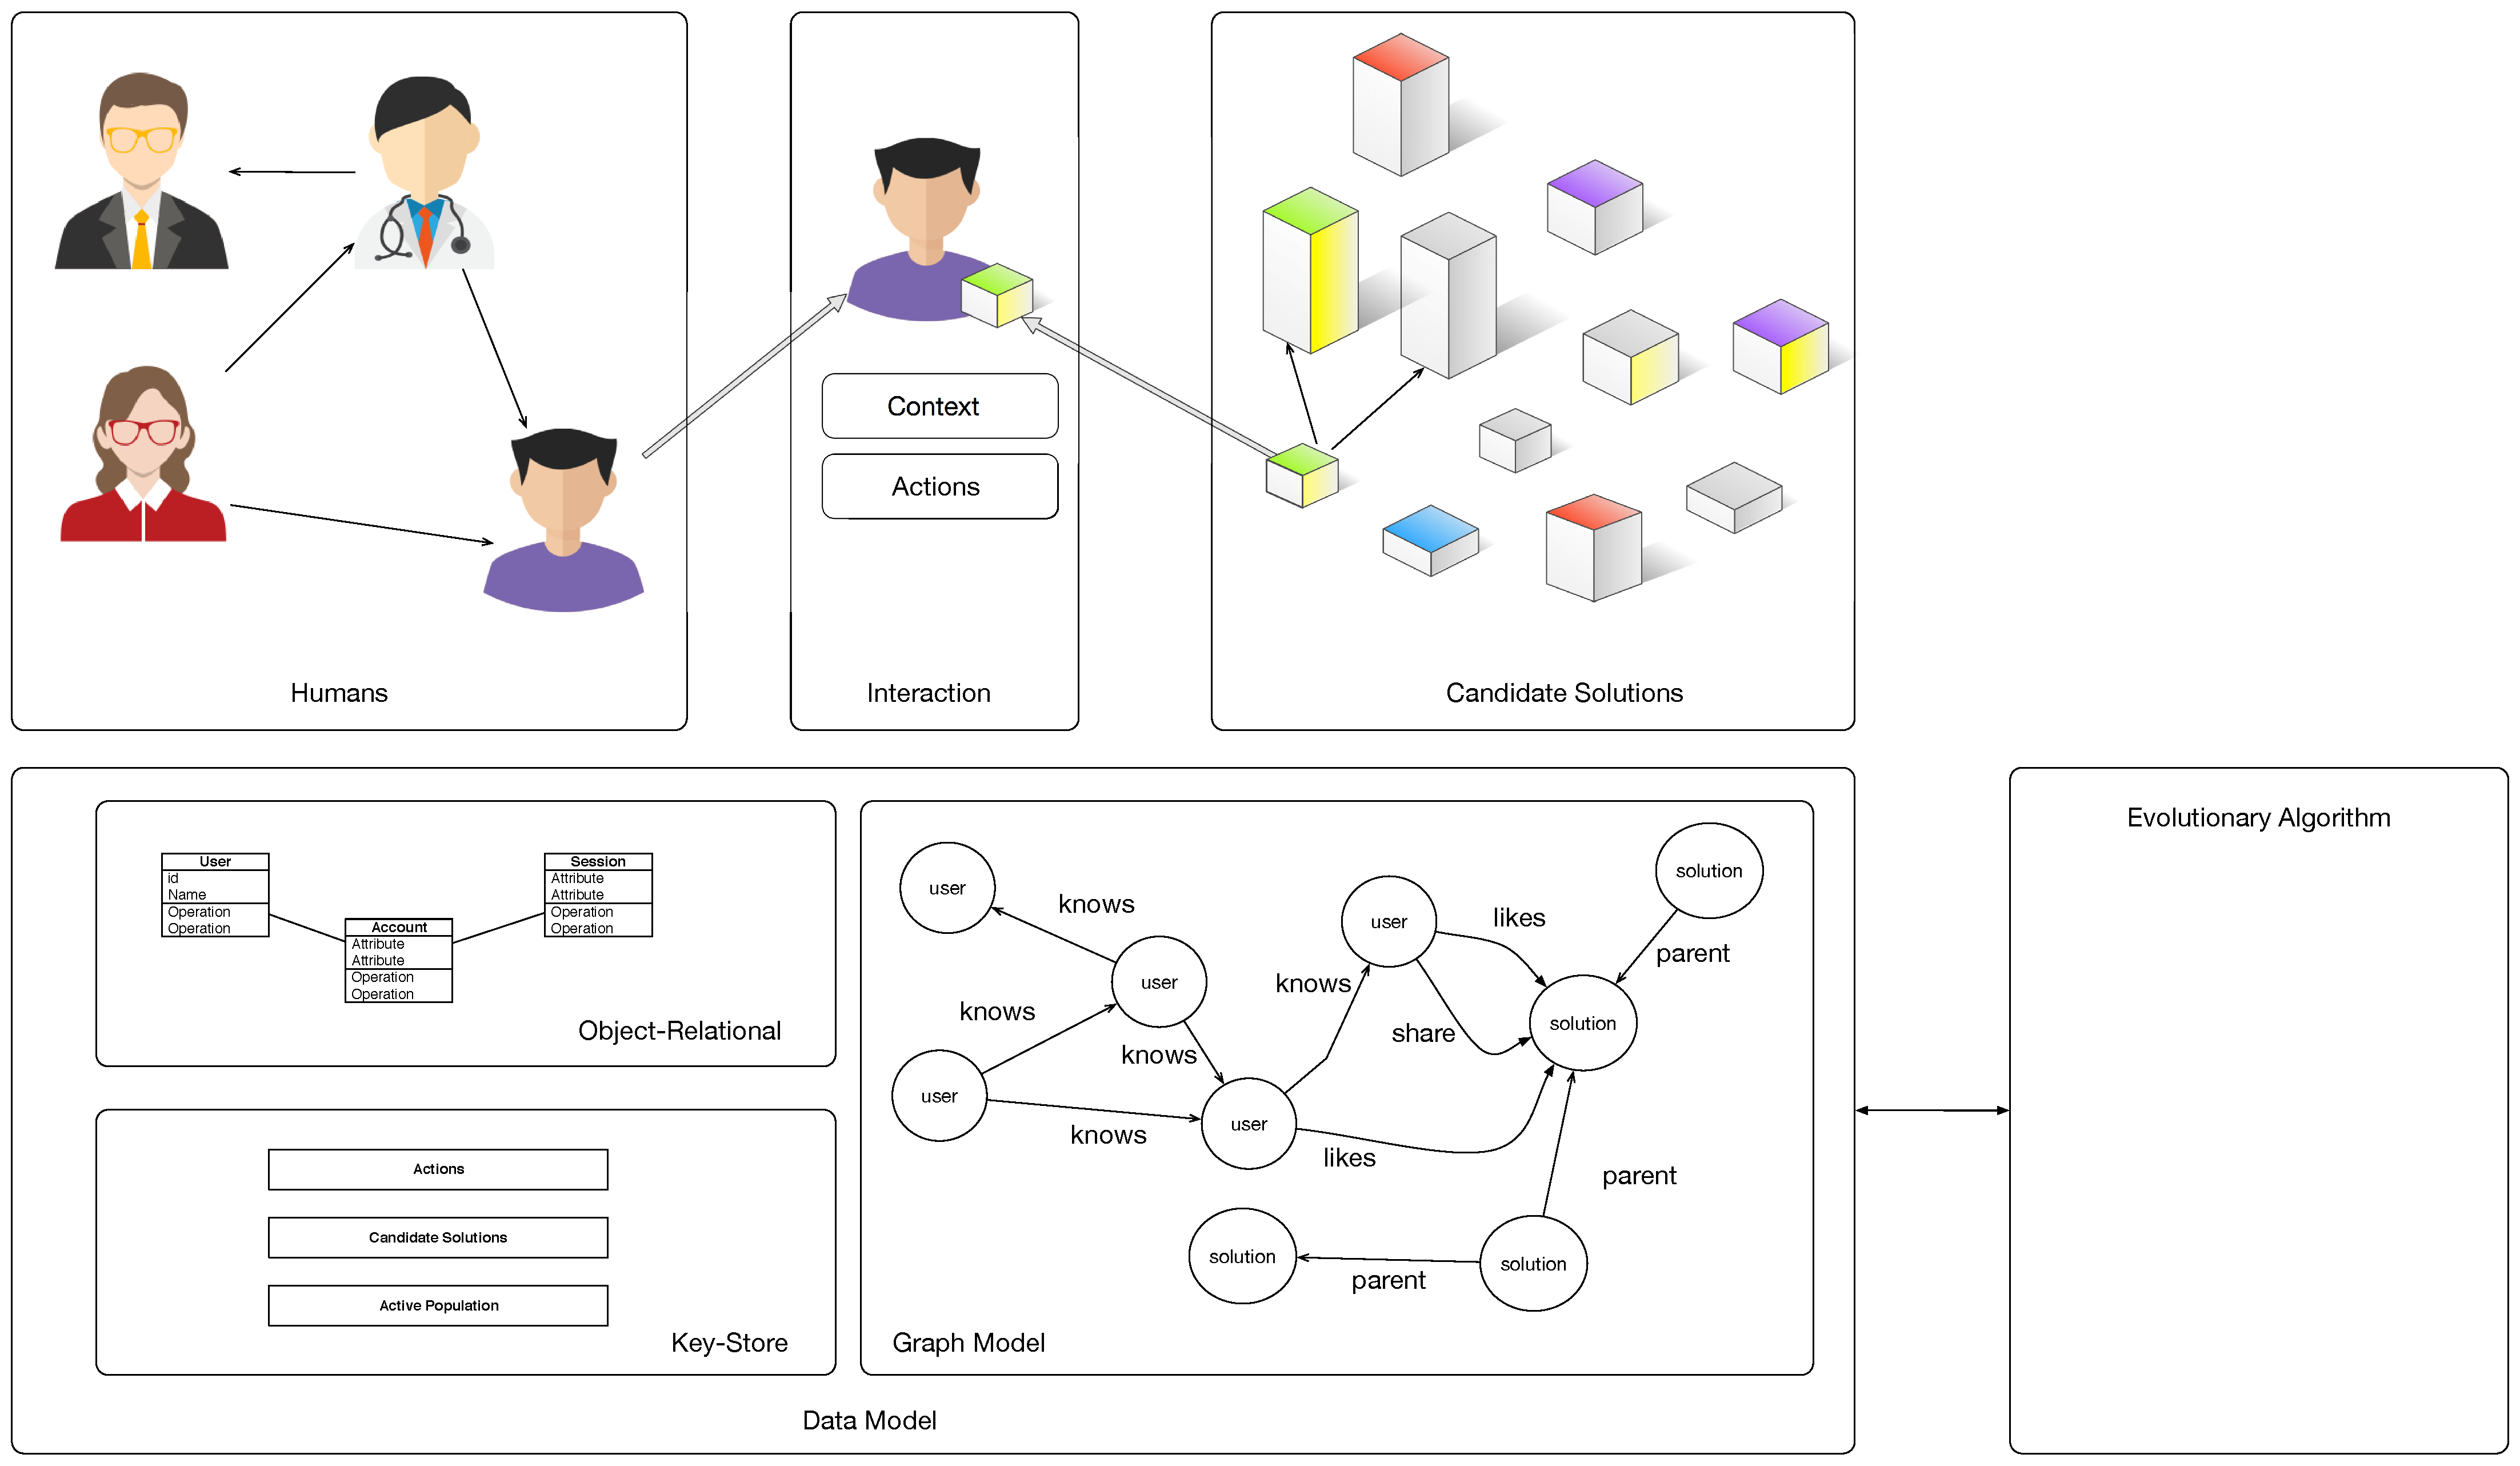
\includegraphics[width=6in]{img/framework.eps}
    \caption{IEC Human-centered framework.}
    \label{fig:hc_framework}
\end{figure*}

\section{Human-Centered C-IEC Framework}
\label{sec:framework}
% You have to clearly express the objectives of the paper from tine
% introduction. If the objective is to reduce fatigue via social
% engagement, you have to frame the results that way.
% Ok, added - Mario 
The general goal of this research is to develop a human-centered \cite{gasson2003human} 
software framework that can be used to increase volunteer participation 
in C-IEC systems. A framework is defined as a reusable architectural design together
with an implementation \cite{campbell1991choices}, in this case 
providing generalized components to developers and researchers of C-IEC systems. 
The proposed framework includes components that can be refined to increase
participation and also to minimize the amount of evaluations needed for the evolutionary 
process in a given IEC application. Software frameworks often have 
a vision \cite{carneiro2010introducing} guiding their
design. Before diving into details the main design considerations of the
framework are explained next: 

\begin{itemize}
\item {\bf Users are human.} 
  The framework follows the approach of human centered computing \cite{sebe2010human},
  in which the context, environment, interfaces, preferences, accessibility, human relations,
  cognitive limitations, culture, creativity and other human aspects are an integral part 
  of the system. Humans are the computing resources of the system, having unique characteristics
  as those identified by Sun \& Dance \cite{Sun2013}:
\begin{quote}
  (1) humans can solve computer hard problems; (2) humans are very good at exception handling,
  (3) humans have creativity, (4) humans have cognitive load limitation, (5) humans are
  vulnerable to psychological manipulation, (6) humans are prone to errors,
  especially for reflective tasks.
\end{quote}  

\item {\bf Users are volunteers.} Users donate their computing resources, so they are 
unaccountable, sometimes they try to game the system. Project owners must actively promote and
design the interactive system to engage volunteers \cite{oh2015clicking}. % Define
\item {\bf Users are not alone}
  Relationship between users in an interactive evolutionary algorithm can be modeled
  as a social network, with well established semantics, algorithms and metrics 
  \cite{ahuja1993network}.
  A graph model could enable researchers to find other ways of identifying leaders of 
  opinion or measuring the similarity between user's preferences. 
  These measures can then be used by recommender algorithms selecting 
  phenotypes according users' preferences. 

\item {\bf Context of use matters.}
  Fischer \cite{fischer2012context}
  defines context as
  \begin{quote}
  the interaction between humans and
  computers in socio-technical systems that takes place in a certain
  context referring to the physical and social situation in which
  computational devices and environments are embedded.
\end{quote}   
  Fischer also identifies the important aspects to consider when the context is used: how is
  contextual data obtained, how is context represented and what
  goals and purposes the context has when it is used in a particular
  application. An IEC system will  be used within a certain range 
  of technical, physical and social or
  organizational environments \cite{maguire2001context} that may affect its use.
 
\item {\bf Interaction is a stream of actions.}
  Real time processing of users' actions could be needed for certain applications when data is 
  captured by sensors, or directly captured as user input. For example, social networks keep
  track of users' interactions with other users, media objects and places. Users of 
  social networks (for instance the Facebook Graph) are accustomed to express these 
  complex relationships in sentences such as: ``John and Ann eating breakfast at Tony's''. 
  Other example is the W3C Activity Streams 2.0 specification used for representing activities 
  common in social web applications \cite{json:streams}. 
\end{itemize}

The above considerations have guided the design of the framework, and throughout they have been
treated as application constraints. In order to satisfy theses requirements the
human centered IEC architecture consists of three high level components depicted
in figure \ref{fig:hc_framework}:

\begin{enumerate}
  \item {\bf Interactive System.} 
  This is the real world system that we are going to represent in the data model, 
  it consist of human users and their interactions with one or more phenotypes
  from the population. There are many ways in which humans could interact 
  with these phenotypes. The interaction consists of a set of actions and 
  takes place in a certain context; for example, through a mobile device  
  or by interacting with real world objects 
  \cite{de2014artists,de2013unplugging}. 
  There is also the possibility that fitness or even part of the search 
  is done by devices lent by humans \cite{DBLP:conf/gecco/MereloCGCRV16}.
  The information gathered through the interaction is the primary focus
  as it will guide the search. 

  \item {\bf IEC Data Model.}
  A data model is used to describe the IEC system prior to a physical 
  implementation.  Depending on the domain several techniques can be used.
  Parts of the system could be better described by an entity-relationship 
  modeling, to be used in a relational database or a class digram for a 
  key-value store. A graph is proposed for modeling the social network of users 
  and their interaction with the population. When implemented, a graph database 
  will be the back-end of the system. 

  \item {\bf Evolutionary Algorithm.} 
  The Evolutionary Algorithm (EA) algorithm interacts 
  with the data model. The EA could also be run with the help of
  humans, for instance in the XY project \cite{de2013unplugging} artists actually painted
  the solutions of the new population and applied every genetic operator.
\end{enumerate}

\section{Data Model Implementation}
\label{sec:implementation}

The core of the framework is the data model because both the IEC system and the EA will 
depend on the application. In this section implementation details of the Data Model are presented.
Three database models are employed to store different elements of the system: 

\begin{itemize}
\item {\bf EvoSpace-Redis.} 
EvoSpace is a population store \cite{Evospace}  for the development of 
evolutionary algorithms that are intended to run on a cloud computing model. 
The population is decoupled from any particular evolutionary algorithm. 
Candidate solutions are stored as of objects in a population, and they can be withdrawn, 
processed and replaced using a specified set of methods \cite{GValdez2015}. The population
is stored in-memory, using the Redis key-value database. Redis was chosen over a relational 
database management system because it provides a hash based implementation of sets and 
queues which are natural data structures for the EvoSpace model. Basically, a sample of 
candidate solutions are retrieved from the server, evaluated and then sent back. 
The same operations are used to evolve the population. In EvoSpace individuals replaced 
in the population are stored indefinitely, to permit users to store permalinks to them.
Implementation details are presented in \cite{garcia2013evospace}.

\item {\bf Graph-Neo4J.} 
 Collaborative IEC (C-IEC) systems need to store highly connected data, as it is common 
 in current applications like social networks. In order to deal with large datasets of connected 
 data found in these systems, graph databases \cite{angles2012comparison} have been proposed 
 as an alternative to relational databases which have performance limitations when dealing with 
 highly connected data \cite{holzschuher2013performance}.
 A graph is proposed for modeling the social network of users, their interaction with 
 candidate solutions, and the relationships between them in the population.
 The graph database system used in the implementation is Neo4J, which is
 a scalable solution \cite{miller2013graph,holzschuher2013performance}, well 
 supported and documented in PaaS infrastructures like Heroku. The Cypher query 
 language it used to retrieve views from the graph.
 An example query is shown in Figure \ref{fig:cypher} where the relations 
 between users and solutions are presented.
  
  \begin{figure}[!t]
    \centering
        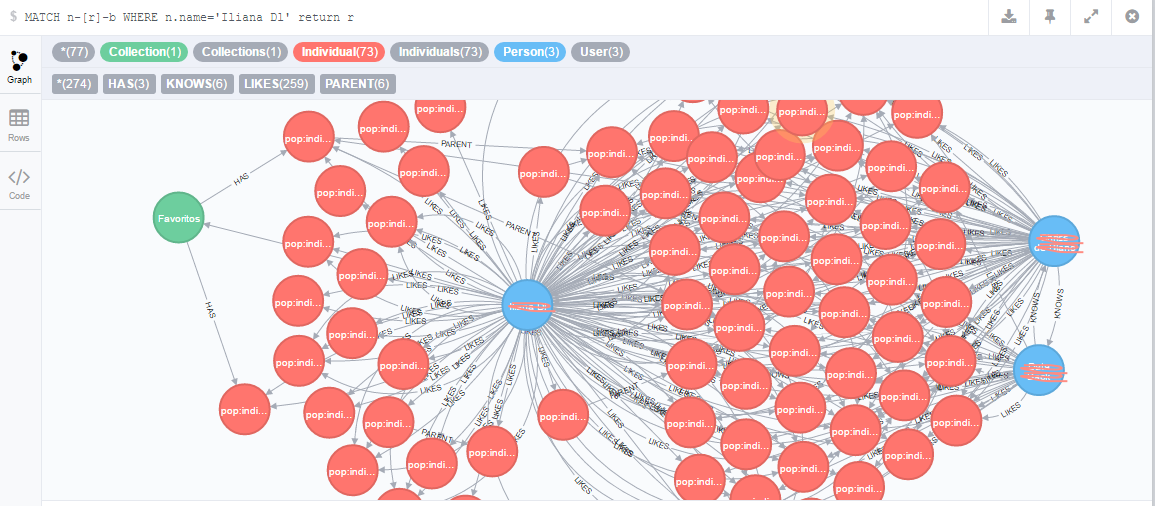
\includegraphics[width=3.5in]{img/gui-neo.png}
    \caption{Example query in Cypher.}
    \label{fig:cypher}
  \end{figure}

\item {\bf Relational Objects-PostgreSQL.}
  The PostgreSQL relational database system is also employed because user 
  sessions and authentication,
  as well as dynamic web pages are handled directly by the Django web
  framework \cite{garcia2013evospace}. % these implementations details
                                % could go if needed. 


\item {\bf Interfaces.}
The appropriate human interface will depend on the application domain, 
the current framework implementation employs a web based application. Developers 
can use different templates, to present one or more phenotypes 
at a time, and the type of rating system:  based on ``likes'' or in a rating from one to five (stars). 
Other implementations do not need a graphical interface at all, for example the
EvoDrawings installation or the XYZ Project \cite{de2014artists}.   

\item {\bf Evolution.}    
The EA is decoupled from the data model, the algorithm 
could be implemented as an EvoWorker \cite{garcia2013evospace}, use an external library, 
or even assigned to humans. An additional tool was implemented for a human based evolution, 
where volunteers select the parents of the next generation and upload the 
new individuals \cite{de2014artists}.  
\end{itemize}

\section{Case Study: EvoDrawings}
\label{sec:evodraw}
As a case study, a C-IEC application was developed using the 
EvoSpace-Interactive (ES-I) platform \cite{garcia2013evospace}
A brief description of the application is presented next, focusing
on the data elements that where ported to the graph model.

\begin{figure}[!t]
    \centering
        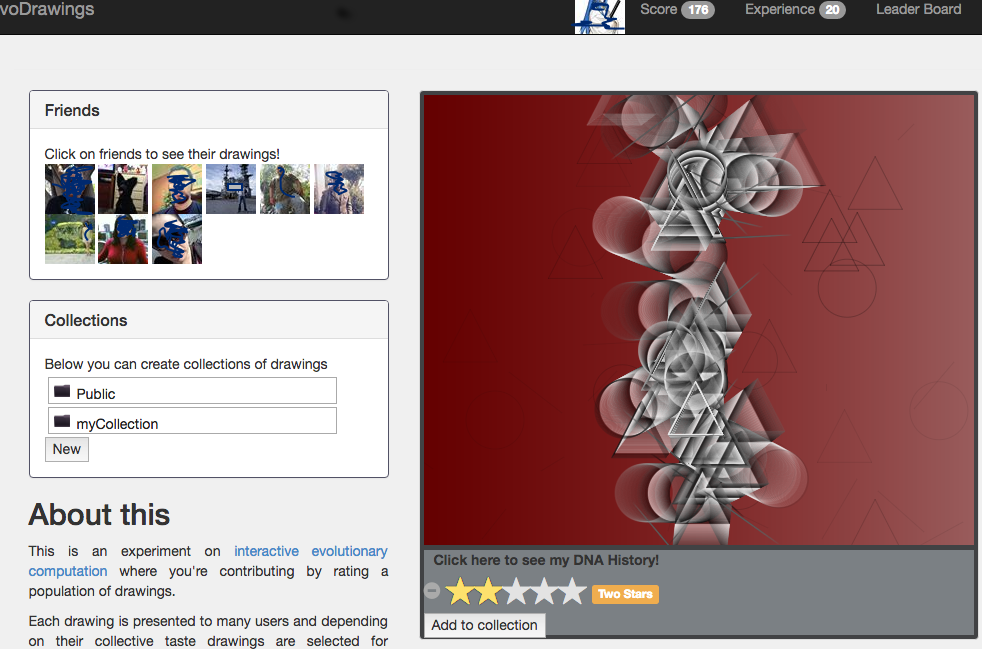
\includegraphics[width=3.5in]{img/interface.png}
    \caption{User interface of the EvoDrawings application.}
    \label{fig:web}
\end{figure}

\subsection{Fitness Assignment}
The ES-I platform has been programmed to employ a 
collaborative methodology for performing fitness assignment. 
Several registered users assign a quality assessment to a single
phenotype and then an aggregated fitness value is calculated,
depending on the rating (from 1 to 5 stars) by each particular user,  
resulting in a many-to-many relationship between users and
phenotypes. Other components or users of the systems can 
query this user-phenotype relation to extract relevant
knowledge about the process and the population. For instance, showing the
most popular phenotype, or the user with more participation 
\cite{picbreeder}.
In order to do this, meta-data about phenotypes 
must be permanently stored, even
if they are no longer in the active population. 

\subsection{Collaboration}
\label{sec:col}
Users need to authenticate themselves to the system using their
Facebook account. In that sense, some users might not be interested
either because they do not want to give that information or simply because
they do not use that social network. Even if we might lose
some users that way, the additional information we obtain for scoring
phenotypes more than balances that. 
After logging in,
users can collaborate with their Facebook friends, 
sharing the phenotypes they like, or by taking phenotypes
from their friend's collections by using the web interface depicted 
in Figure \ref{fig:web}.
At the top left corner a list of Facebook friends is presented
to encourage users to interact with the system. In the central 
\emph{ Wall } area, a phenotype sampled from the population that is
being evolved via the evolutionary algorithm 
is shown to the user.
Here, the user can interact with the system in two ways.
First, he can assign a rating to the phenotype or choose to add an image to one of their \emph{Collections}.
A collection is a special folder that stores those phenotypes a user likes and wishes
to save. After the user finishes interacting with the phenotype
on the Wall, he can choose to retrieve a new one from the population.
At the left hand side of Figure \ref{fig:web}, the web page shows the \emph{Collections} section.
The user can create several collections, to group and organize his favorite 
artifacts. Moreover, users can browse the content of each collection and from
there share images through their social network. This makes the assignment 
of fitness through the rating system a {\em social} activity, 
pursuing the objective of this work, which is to increase user engagement.

\subsection{Graph Model} 
The graph model for the EvoDrawings application has the following types of
nodes: {\bf User}, {\bf Phenotype} and {\bf Collection} . The Collection node represents
a collection of drawings belonging to users. One collection can contain many phenotypes 
or be empty. A single phenotype could be shared by many collections. The interaction 
between these entities are represented by the following edges:

\begin{itemize}
\item {\bf Likes} This relation describes the interaction between a user and
a phenotype in which a rating value is assigned.

\item {\bf Knows} The relation connects two users that know each
other in the Facebook social graph. 

\item {\bf Parent} Describes what phenotype is the parent of a new
  phenotype. 

\item {\bf Has} The relation describes an ownership relation between users and
those collections they own. 
\end{itemize}
% Once again, these implementation details could go - JJ

\subsection{Gamification}
The rewarding mechanism as it is applied in EvoDrawings gives more importance 
to the preference of those users with higher reputation
as given by their score points and experience levels.  
Each time a user does on of these actions their score is incremented by one:
start a session, rate a phenotype, create a collection, save a phenotype of 
the wall to a collection, save a phenotypes from a friend's collection, and
explore collections of other friends.

Two variables are used to determine the weight of a user's preference:
\begin{itemize}
\item {\bf Experience}: This variable depends on the score and is a value 
between 0 and 100. A new user starts at zero, and the experience increases until
it reaches 100 actions. It is assumed for this case, that once a user
reaches this value, it has enough experience on using the
application. % What happens before that? - JJ  
% explained - Mario
\item {\bf Participation}: This variable is simply the degree of the user node 
in the graph (number of edges).    
\end{itemize}

\section{Experimental Setup}
\label{sec:experiment}

Three versions of EvoDrawings were compared:
\begin{itemize}
\item Base (B): All users have the same weight.
\item Non Graph Gamification (G): Only experience is considered.
\item Graph Gamification (GG): Both experience and participation are considered.
\end{itemize}
When gamification was employed, all score values known where presented to users
and a ranking of users by weight was shown in a window. Table \ref{tab:params} shows 
the parameters used for the evolutionary algorithm. 

\begin{table}
  \small
  \caption{ Parameters for experiments.  }
  \label{tab:params} 
  \centering
  \small
  \begin{tabular}{l  c}
    \hline\noalign{\smallskip}
     Parameter & Value \\
    \noalign{\smallskip}\hline\noalign{\smallskip}
    Initial Population Size   & 80 \\ \hline
    Sample Size & 1 \\ \hline
    Step Size & 8 Samples \\ \hline
    Mutation &  \\ \hline
    Selection & Tournament \\ \hline
    Tournament Size &  6 \\ \hline
  \end{tabular}
\end{table}

% Anuncements
At the start of every experiment, a call to participation was issued
through social networks.  The link used in the call for participation
was a shortened Google URL, that provides meta-data and analytics for the
users that click on it. 
 %Will we comment on that? - JJ
 % To do.
  In Table \ref{tab:urls} the URL for each 
deployment in the Heroku platform is shown,
along with the short URL and the analytics link. In the same table a link to the GitHub 
application repository used to deploy to Heroku is also listed. Only data 
for the first week of deployment was considered for the experiments, and they where conducted 
between January and May of 2016. 

\section{Results}
\label{sec:results} 
Before release, each deployment was first tried with a few beta testers. 
When applying the leader board gamification technique for the first time a 
problem was found: some users were cheating by giving a
rating to an animation even before it was returned from the server, this was done by just
constantly clicking the mouse button. This is a common problem found in systems using leader
boards because by making the scores visible to other players they are encouraged 
to compete \cite{hickman2010total}. The final version disabled the button until 
the drawing animation was over. The results of each of the three experiments in 
terms of participation are detailed next.

\begin{table}
  \small
  \caption{After a week of the announcement the total number of volunteers, 
  nodes and edges in the graph and analytics URLs}
  \label{tab:urls} 
  \centering
  \small
  \begin{tabular}{l l l l l}
    \hline\noalign{\smallskip}
     Deployment &  Users &  Nodes &  Edges & URL \\
    \noalign{\smallskip}\hline\noalign{\smallskip}
    B   & 53 &  595   & 2220  & goo.gl/jLis4Q.info \\ \hline
    G   & 54 &  648   & 2596  & goo.gl/jqjNy5.info \\ \hline
    GG  & 68 &  932   & 3594  & goo.gl/J8TCe1.info \\ \hline
    \end{tabular}
\end{table}

Table \ref{tab:urls} shows the total number of volunteers, nodes and edges 
in the graph after each experiment. Moreover, the total number of evaluated 
phenotypes for each volunteer is presented in figure 
\ref{fig:top-ranked-participation} where users are ranked by the 
number of phenotypes they rated. In the \emph{x} axis is the rank and in the \emph{y} axis 
the number of phenotypes evaluated using a logarithmic scale. Results show that when 
considering deployments B and G, the difference came with users with a medium level of participation.
When comparing all the experiments the deployment GG had the higher
number of participation in users of all levels, besides attracting a
bigger number of users.    

\begin{figure}[!t]
    \centering
        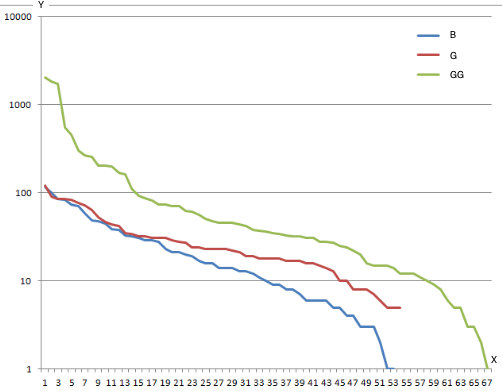
\includegraphics[width=3.3in]{img/comparison.png}
    \caption{Users ranked by the number of phenotypes they 
    rated vs. the number of phenotypes evaluated using a logarithmic scale. }
    \label{fig:top-ranked-participation}
\end{figure}

Moreover, modeling the performance of an C-IEC system
involves understanding its dynamics. Previous works on browser-based
volunteer computing have used basic metrics such as
the number of users or the time spent by every one in the
computation \cite{DBLP:journals/gpem/LaredoBGVAGF14, 2016arXiv160101607M}. 
While works on other platforms such as SETI@home
\cite{javadi2009mining} have found that the Weibull, log-normal, and
Gamma distributions where viable models of the  
the availability of computing resources in several clusters, which  is 
in concordance with the results obtained in \cite{agajaj}, and also
browser-based volunteer evolutionary systems like NodIO \cite{DBLP:conf/gecco/MereloCGCRV16}.
The shape of those distributions is a skewed bell
with more resources in the {\em low} areas than in the high areas; i.e., 
there are many users that give a small amount of cycles, while there
are just a few that give many cycles. In order to assess gamification techniques alongside C-IEC follows the
same pattern, participation was fitted to a 
Weibull distribution,
and shown in Figures \ref{fig:w1} and \ref{fig:w3}, 
confirming  this model for user interaction, although with different fitted
values in each case. A graph query was used to compare the number of volunteers in deployments
B and GG (shown in figures \ref{fig:B-network} and \ref{fig:GG-network} respectively). 

%
\begin{figure}[!t]
    \centering
        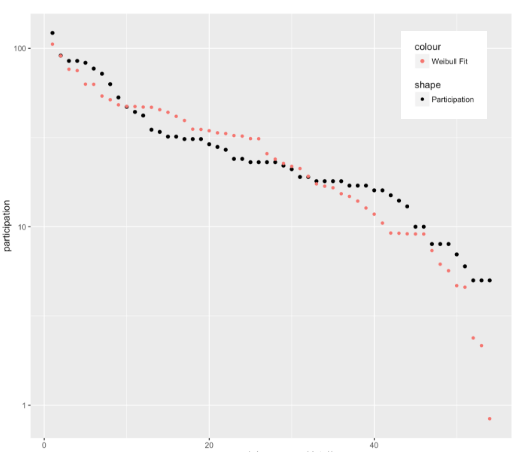
\includegraphics[width=3.2in]{img/weibull_1.png}
    \caption{Deployment B. Weibull Fit.}
    \label{fig:w1}
\end{figure}
%
\begin{figure}[!t]
    \centering
        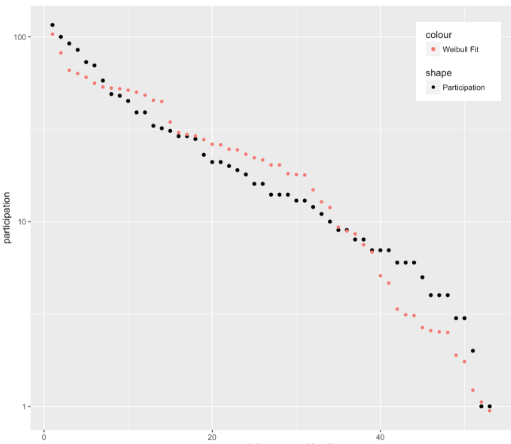
\includegraphics[width=3.2in]{img/weibull_2.png}
    \caption{Deployment G. Weibull Fit.}
    \label{fig:w2}
\end{figure}

\begin{figure}[!t]
    \centering
        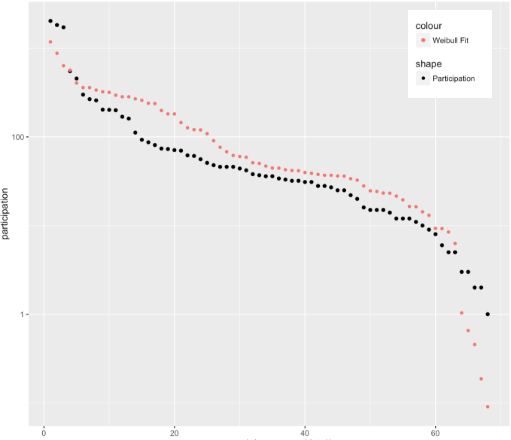
\includegraphics[width=3.2in]{img/weibull_3.png}
    \caption{Deployment GG. Weibull Fit.}
    \label{fig:w3}
\end{figure}





% This has nothing to do with the rest of the paper. You are not
% modeling anything. It's just another application of the
% framework. Could be mentioned in the state of the art, that's
% all. We should devote more space to the study of user interactions. 

% Once again, no model, no relation to the rest of the paper. Either
% you talk about a model of interactions with humans and their
% similarity with the first case study, or you eliminate it. How do
% you tackle boredom? How do you increase engagement? Those are the
% paper's topics, you can't just drop it here because it's interactive
% - JJ
\begin{figure}[!t]
    \centering
        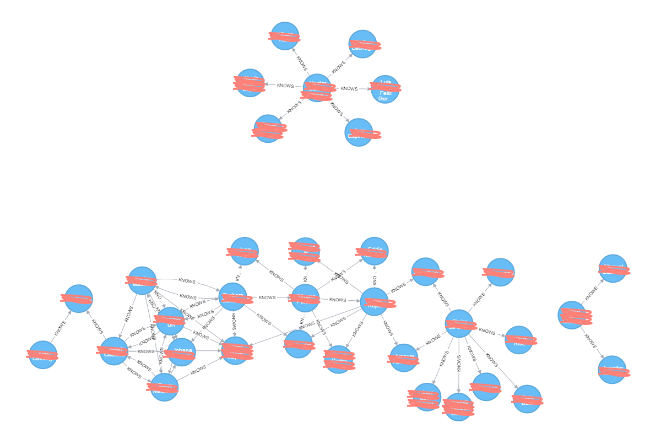
\includegraphics[width=3.2in]{img/user_known_2.png}
    \caption{User network view of the Base deployment}
    \label{fig:B-network}
\end{figure}
\begin{figure}[!t]
    \centering
        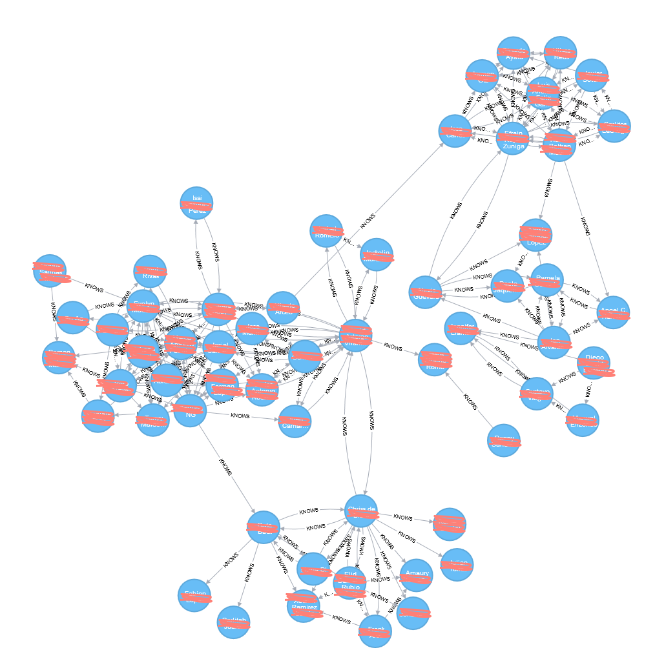
\includegraphics[width=3.2in]{img/user_known_3.png}
    \caption{User network view of the Graph Gamification deployment}
    \label{fig:GG-network}
  \end{figure}
  
\section{Conclusions}
\label{sec:conclusions}

Volunteer-based and C-IEC systems involve the dynamic 
interaction of many entities and artifacts. Employing a human-centered approach 
will allow researchers to understand and visualize this kind of
systems better. % But you would have to provide some proof of this - JJ

In this paper a human-centered software framework was proposed, and was validated
through the implementation and refinement of a C-IEC application.
This framework enabled the implementation of a gamification technique 
to improve engagement in a case study which provides a common arena where users are aware of the
activities of other users in the social neighborhood. 

After applying the gamification techniques user participation follows the
same pattern and was fitted to a Weibull distribution, which matches
results obtained in other browser-based volunteer systems.
% We would have to check the actual coefficients. - JJ

It was shown how the estimation of fitness of candidate solutions
can take advantage of a graph model representation. Also, the graph
offers another view of the system that it would have been
difficult to replicate with a relational database. 
% More conclusions and some way of relating the three case studies
% would be something that is missing and should definitely go here - JJ
% No longer needed as they where removed - Mario

One of the interesting future lines of work would be to look a bit
more closely at the behavior of users as they are rating artifacts 
in the web system. These initial experiments hint at a possible power law, which might indicate that
the IEC system could be self-organizing, a process that would allow it
to reach a critical state, as has been found in software repositories,
for instance \cite{Merelo2016:repomining}. 
The dynamics of this kind of system are fundamentally different, and our future research will
include exploring these aspects of the system. 

Another line of work would be to study the possible negative effects of using  
gamification techniques to improve engagement, like cheating or
literally {\em gaming} the system to defeat competition. We already
found some hints of this behavior at the beginning of the release of
this system, but more subtle effect could be taking place. 
Finally, the refinement of the proposed Human-Centered framework will need
more case studies and further multi-disciplinary research. 

\begin{acks}
  Reserved\\
  Space for acks. 



\end{acks}
